% Copyright 2016 - 2018 Bas van Meerten and Wouter Franssen
%
%This file is part of ssNake.
%
%ssNake is free software: you can redistribute it and/or modify
%it under the terms of the GNU General Public License as published by
%the Free Software Foundation, either version 3 of the License, or
%(at your option) any later version.
%
%ssNake is distributed in the hope that it will be useful,
%but WITHOUT ANY WARRANTY; without even the implied warranty of
%MERCHANTABILITY or FITNESS FOR A PARTICULAR PURPOSE.  See the
%GNU General Public License for more details.
%
%You should have received a copy of the GNU General Public License
%along with ssNake. If not, see <http://www.gnu.org/licenses/>.

\documentclass[11pt,a4paper]{article}
% Copyright 2016 - 2017 Bas van Meerten and Wouter Franssen
%
%This file is part of ssNake.
%
%ssNake is free software: you can redistribute it and/or modify
%it under the terms of the GNU General Public License as published by
%the Free Software Foundation, either version 3 of the License, or
%(at your option) any later version.
%
%ssNake is distributed in the hope that it will be useful,
%but WITHOUT ANY WARRANTY; without even the implied warranty of
%MERCHANTABILITY or FITNESS FOR A PARTICULAR PURPOSE.  See the
%GNU General Public License for more details.
%
%You should have received a copy of the GNU General Public License
%along with ssNake. If not, see <http://www.gnu.org/licenses/>.

\usepackage[british]{babel}
\usepackage{graphicx,booktabs,listings,amsmath,pgfplots,pgfplotstable}
\usepackage[small,bf,nooneline]{caption}
\usepackage{subcaption}
\usepackage[sort&compress,numbers]{natbib}
\usepackage{tikz}
\usepackage{mathtools}
\usepackage[nottoc]{tocbibind}%adds bibliography to table of contents.
\graphicspath{{./images/}}
%\setlength{\textwidth}{453pt} %597 pt is the a4 paperwidth. Minus 2 in margin. 72 pt = 1 in
%\setlength{\hoffset}{-\oddsidemargin}
%\setlength{\voffset}{-30pt} %
%\setlength{\textheight}{651 pt} %a4 height 845 pt minus 2* total headheight. In this case 2*88pt
%% examine margines via the layout package. Use command \layout{} in document to draw a picture.
%\setlength{\parindent}{0.5 cm}
%\setlength{\parskip}{0 cm}
\usepackage[left=82pt,right=82pt,top=95pt,bottom=95pt,footnotesep=0.5cm]{geometry}
%\setlength{\headheight}{14pt}

%define colours--------------------
%dark
\usepackage{xcolor}
\definecolor{MyGrayD}{RGB}{1,1,1}
\definecolor{MyRedD}{RGB}{237,45,46}
\definecolor{MyGreenD}{RGB}{0,140,71}
\definecolor{MyBlueD}{RGB}{24,89,169}
\definecolor{MyOrangeD}{RGB}{243,125,34}
\definecolor{MyPurpleD}{RGB}{102,44,145}
\definecolor{MyBrownD}{RGB}{161,29,32}
\definecolor{MyPinkD}{RGB}{179,56,147}
%normal
\definecolor{MyGray}{RGB}{114,114,114}
\definecolor{MyRed}{RGB}{241,89,95}
\definecolor{MyGreen}{RGB}{121,195,106}
\definecolor{MyBlue}{RGB}{89,154,211}
\definecolor{MyOrange}{RGB}{249,166,90}
\definecolor{MyPurple}{RGB}{158,102,171}
\definecolor{MyBrown}{RGB}{205,112,88}
\definecolor{MyPink}{RGB}{215,127,179}
%light
\definecolor{MyGrayL}{RGB}{204,204,204}
\definecolor{MyRedL}{RGB}{242,174,172}
\definecolor{MyGreenL}{RGB}{216,228,170}
\definecolor{MyBlueL}{RGB}{184,210,235}
\definecolor{MyOrangeL}{RGB}{242,209,176}
\definecolor{MyPurpleL}{RGB}{212,178,211}
\definecolor{MyBrownL}{RGB}{221,184,169}
\definecolor{MyPinkL}{RGB}{235,191,217}
%----------------------------------

%Figure ref with hyperref
\newcommand{\fref}[1]{\hyperref[#1]{Figure \ref*{#1}}}
\newcommand{\sref}[1]{\hyperref[#1]{Section \ref*{#1}}}
\newcommand{\tref}[1]{\hyperref[#1]{Table \ref*{#1}}}

%Makes a new command for figures with input values: filename, width(times linewidth),
% caption and label.
\newcommand{\onefigure}[4]{
\setlength{\captionwidth}{#2\linewidth}
\begin{figure}
\includegraphics[width=#2\linewidth]{#1}
\centering
\parbox{\linewidth}{\caption{#3}
\label{#4}}
\end{figure}
}

%Makes a new command for tikz figures with input values: tikz commands, 
% caption and label.
\newcommand{\onetikz}[3]{
\settowidth{\captionwidth}{#1}
\ifthenelse{\lengthtest{\captionwidth<0.7\linewidth}}{\setlength{\captionwidth}{0.7\linewidth}}{}

\begin{figure}
\centering
#1
\centering
\parbox{\linewidth}{\caption{#2}
\label{#3}}
\end{figure}
}

%Makes a new command for two figures next to each other with input values: filename1, caption1, label1,filename2, caption2 and label2. Figure width is set to 0.47\linewidth and the space between the figures is filled with \hfill so the sides of the figures align with to edge of the line.
\newcommand{\twofigure}[6]{
\setlength{\captionwidth}{\linewidth}
\begin{figure*}[ht!]
\begin{minipage}[t]{0.47\linewidth}
\includegraphics[width=\linewidth]{#1}
\centering
\caption{#2}
\label{#3}
\end{minipage}
\hfill
\begin{minipage}[t]{0.47\linewidth}
\centering
\includegraphics[width= \linewidth]{#4}
\centering
\caption{#5}
\label{#6}
\end{minipage}
\end{figure*}
}


%Makes a new command for a table with caption witdh equal to the total table width. Input: tabular, caption and label. Example:
%\onetable{
%\begin{tabular}{ccc}
%a&b&c\\
%\hline
%1&1&1\\
%1&1&1\\
%1&1&1\\
%\end{tabular}
%{The caption.}
%{tab:table1}
%}
\newcommand{\onetable}[3]{
\settowidth{\captionwidth}{#1}
\ifthenelse{\lengthtest{\captionwidth<0.7\linewidth}}{\setlength{\captionwidth}{0.7\linewidth}}{}
\begin{table}
\caption{#2}
\vspace{-0.24cm} %Puts caption close to toprule
\label{#3}
\centering
#1
\end{table}
}

%Makes a long table with captionwidth equal to tablewidth. It takes the following arguments:
%1: Column specifier (e.g. cccc)
%2: Caption
%3: Label
%4: First head (i.e. first row of regular table)
%5: Head of consecutive pages
%6: Foot of pagebreak
%7: Lastfoot (e.g. \midrule)
%8: Body of table
\newcommand{\onelongtable}[8]{
\begin{center}
\settowidth{\captionwidth}{
\begin{tabular}{#1}
#4
#8
\end{tabular}} % This ends the captionwidth part. Next comes the real table.

\begin{longtable}{#1}
\caption{#2}\\
\vspace{-0.74cm} %Puts caption close to toprule
\label{#3}\\

#4
\endfirsthead

#5
\endhead

#6
\endfoot

#7
\endlastfoot

#8
\end{longtable}
\end{center}}




%1:pgfplots code
%2:width
%3:caption
%4:label
\newcommand{\pgfplotsfigure}[4]{
\pgfplotsset{width=#2\linewidth}
\setlength{\captionwidth}{#2\linewidth}
\begin{figure}[t]
\centering
#1
\centering
\parbox{\linewidth}{\caption{#3}
\label{#4}}
\end{figure}
}


\usepackage[bitstream-charter]{mathdesign}
\usepackage[T1]{fontenc}
\usepackage[protrusion=true,expansion,tracking=true]{microtype}
\pgfplotsset{compat=1.7,/pgf/number format/1000 sep={}, axis lines*=left,axis line style={gray},every outer x axis line/.append style={-stealth'},every outer y axis line/.append style={-stealth'},tick label style={font=\small},label style={font=\small},legend style={font=\footnotesize}}
\usepackage{colortbl}
\usetikzlibrary{calc}

%Set section font
\usepackage{sectsty}
\allsectionsfont{\color{black!70}\fontfamily{SourceSansPro-LF}\selectfont}
%--------------------


%Set toc fonts
\usepackage{tocloft}
%\renewcommand\cftchapfont{\fontfamily{SourceSansPro-LF}\bfseries}
\renewcommand\cfttoctitlefont{\color{black!70}\Huge\fontfamily{SourceSansPro-LF}\bfseries}
\renewcommand\cftsecfont{\fontfamily{SourceSansPro-LF}\selectfont}
%\renewcommand\cftchappagefont{\fontfamily{SourceSansPro-LF}\bfseries}
\renewcommand\cftsecpagefont{\fontfamily{SourceSansPro-LF}\selectfont}
\renewcommand\cftsubsecfont{\fontfamily{SourceSansPro-LF}\selectfont}
\renewcommand\cftsubsecpagefont{\fontfamily{SourceSansPro-LF}\selectfont}
%--------------------

%Define header/foot
%\usepackage{fancyhdr}
%\pagestyle{fancy}
%\fancyhead[LE,RO]{\fontfamily{SourceSansPro-LF}\selectfont \thepage}
%\fancyhead[LO,RE]{\fontfamily{SourceSansPro-LF}\selectfont \leftmark}
%\fancyfoot[C]{}
%--------------------

%remove page number from first chapter page
%\makeatletter
%\let\ps@plain\ps@empty
%\makeatother
%----------------------

\usepackage[hidelinks,colorlinks,allcolors=black, pdftitle={CSA pattern fitting in ssNake},pdfauthor={Wouter M.J.\ Franssen}]{hyperref}

\interfootnotelinepenalty=10000 %prevents splitting of footnote over multiple pages
\linespread{1.2}

\title{\color{black}\fontfamily{SourceSansPro-LF}\bfseries CSA pattern fitting in ssNake}
\author{}
\date{\color{black}\fontfamily{SourceSansPro-LF}\bfseries \today}


\begin{document}
%\newgeometry{left=72pt,right=72pt,top=95pt,bottom=95pt,footnotesep=0.5cm}
\microtypesetup{protrusion=true} % enables protrusion

\maketitle

\section{Introduction}
The following will explain how CSA NMR data can be fitted ssNake.
 The
tutorial delivered with the ssNake program is considered as prior knowledge. If you have not yet
studied this, please do so before continuing with this example.

In solid state NMR anisotropic chemical shift interactions (CSA) can be a relevant factor in the
description of a spectrum. While, using fast magic angle spinning, the isotropic term can be easily
established, the size and symmetry of the anisotropy are somewhat harder to determine. As these
spectra can be simulated in a straightforward way, fitting the experimental data is a good way to
establish these values.


\section{Data}
The data in this tutorial was recorded on a Varian 300 MHz machine on glycine powder without the use
of MAS. The spectrum shows the $^{13}$C resonance of the carboxyl group of glycine.


\section{Fitting}
Begin by loading the processed data called \texttt{GlycineStatic.mat} that is delivered with this
tutorial. As this is a chemical shift pattern, we want the x-axis to be in ppm:
\begin{itemize}
  \item In the bottomframe, set \texttt{Axis} to \texttt{ppm}
\end{itemize}
This should show this:
\begin{center}
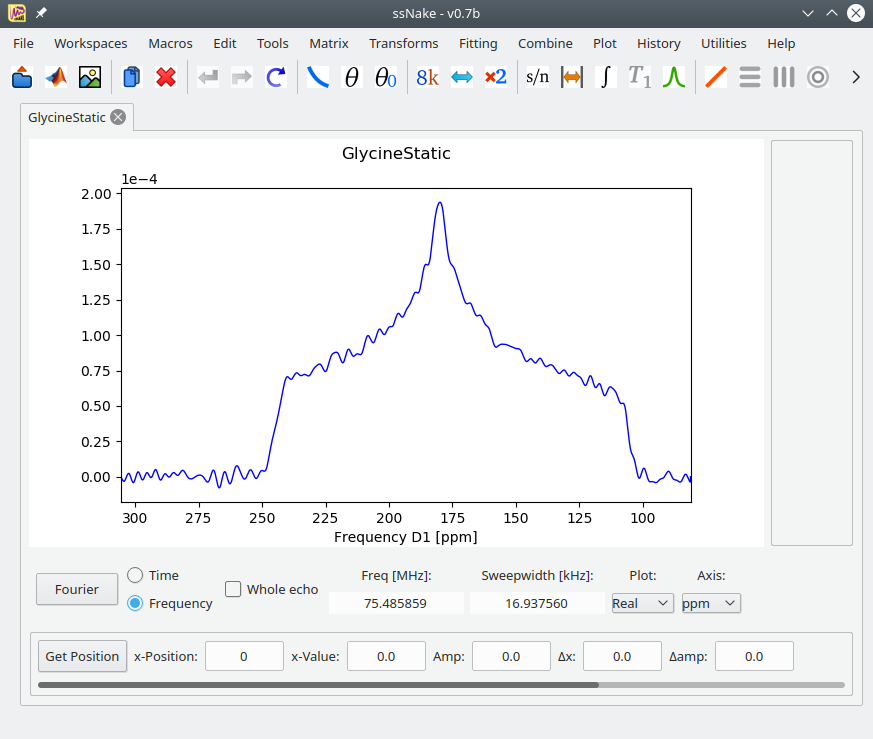
\includegraphics[width=0.8\linewidth]{Figs/Fig1.png}
\end{center}
Which is a nice CSA powder pattern of a static sample. We now need to fit this data to extract the
CSA tensor parameters. Go to \texttt{Fitting $\longrightarrow$ CSA}.

This show the following window:
\begin{center}
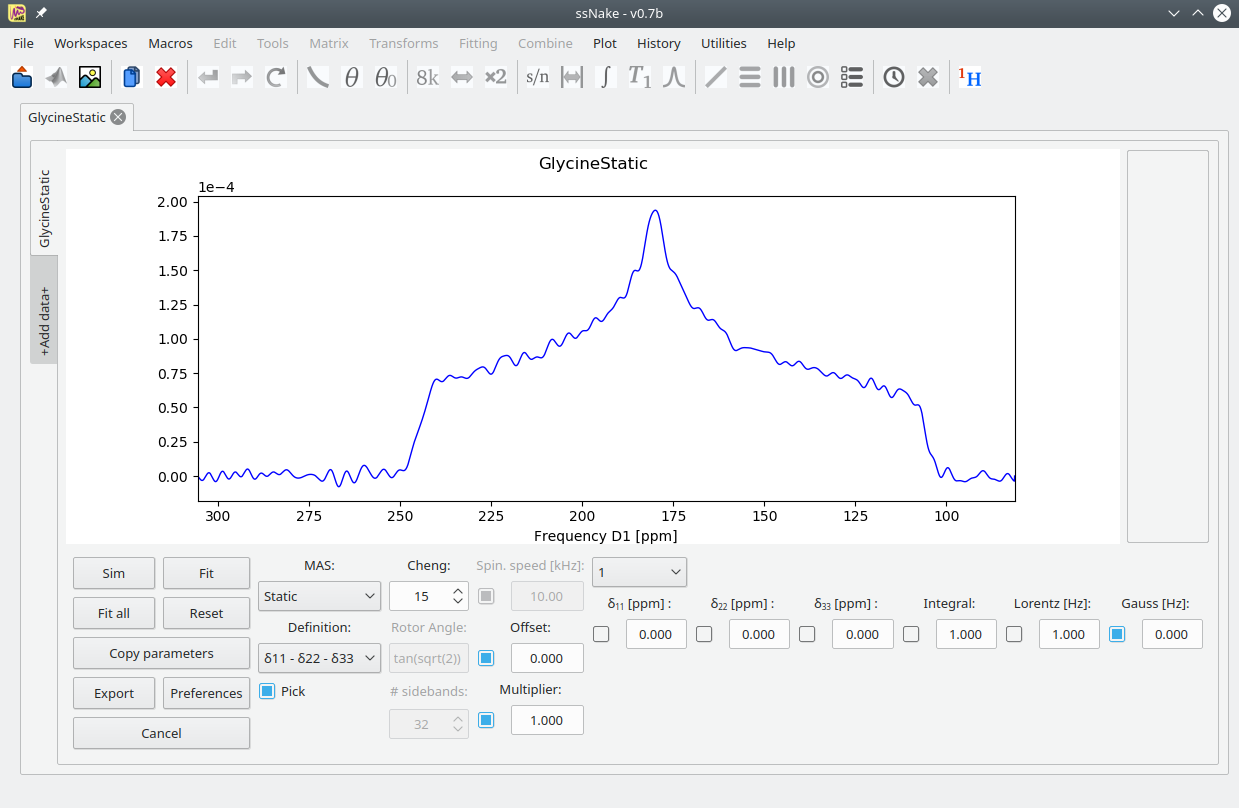
\includegraphics[width=0.8\linewidth]{Figs/Fig2.png}
\end{center}

This window has quite some parameters that we can change. The most important are the boxes on the
right: $\delta_{11}$, $\delta_{22}$, and $\delta_{33}$ are the CSA tensor values. Also shown are some
line broadening parameters (Lorentz and Gauss). The tick boxes next to the input boxes indicate
whether or not the parameters are fixed (checked) or that they may be change during the iterative
fitting (unchecked).

Before we can be an iterative fit, me must first supply some starting values for the fit. This makes
it easier for ssNake to find the best solution. In this CSA fit, this can be easily done by left
clicking on the spectrum: each click sets on of the $\delta$-values to the ppm value under the
cursor. In this case, these values should be equal to the extremities of the powder pattern, and
the `peak' in the center. Left click on the left part of the pattern, the `peak' and the right part.
This should set the $\delta$-values to approximately 243, 181 and 106 ppm, which are good starting
values.

Pushing `Sim' in the left part of the window simulates a spectrum using our current settings. Doing
this leads to:
\begin{center}
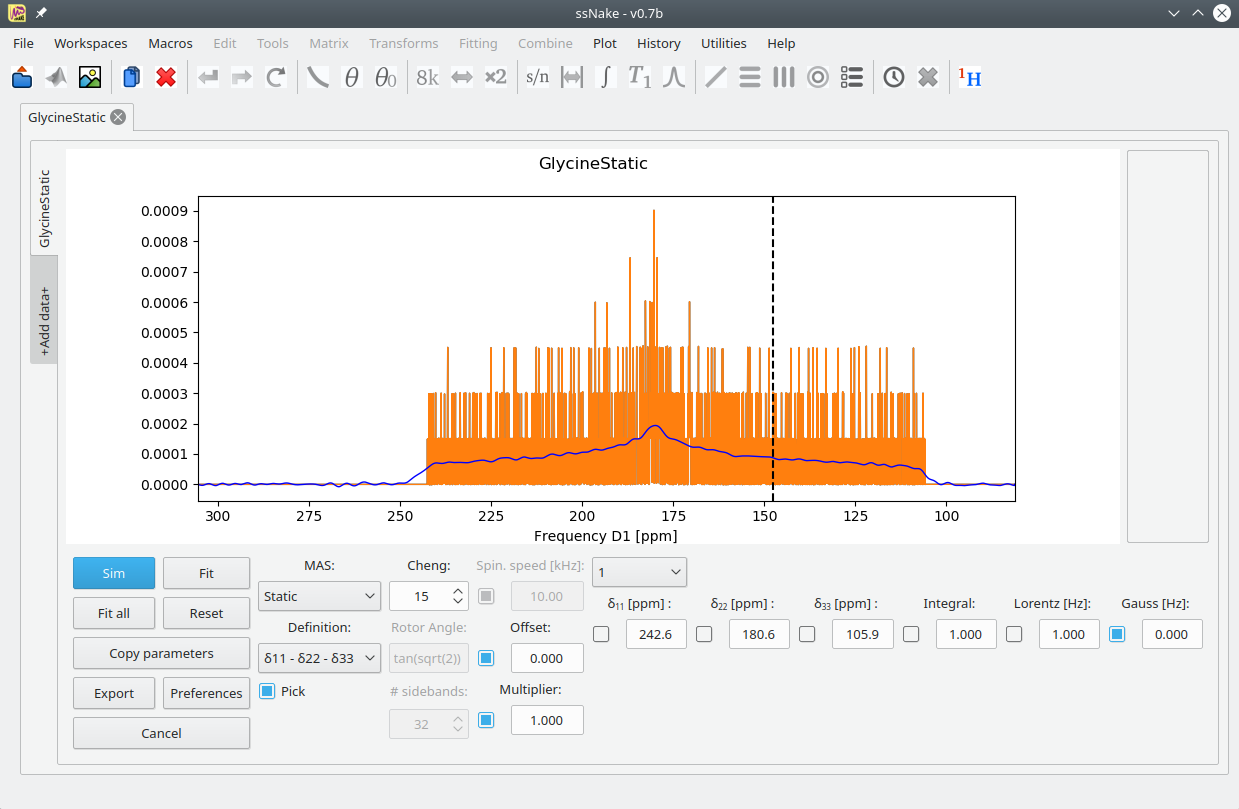
\includegraphics[width=0.8\linewidth]{Figs/Fig3.png}
\end{center}
which looks very ugly. Here the orange line represents the simulated spectrum. The reason why it
looks like this is because the line broadening is quite low (1 Hz), and we only simulate a finite number
of powder orientating. This leads to a series of peaks for each crystal orientation in our synthetic
powder, and not a nice pattern. This issue can be overcome by increasing the number of powder
orientations.
\begin{itemize}
  \item Change the Cheng\footnote{The Cheng number represents the number of orientation to be
	 simulated. It is an exponential scale, so it increases quite fast.} number from 15 to 25
\end{itemize}
Simulating again shows:
\begin{center}
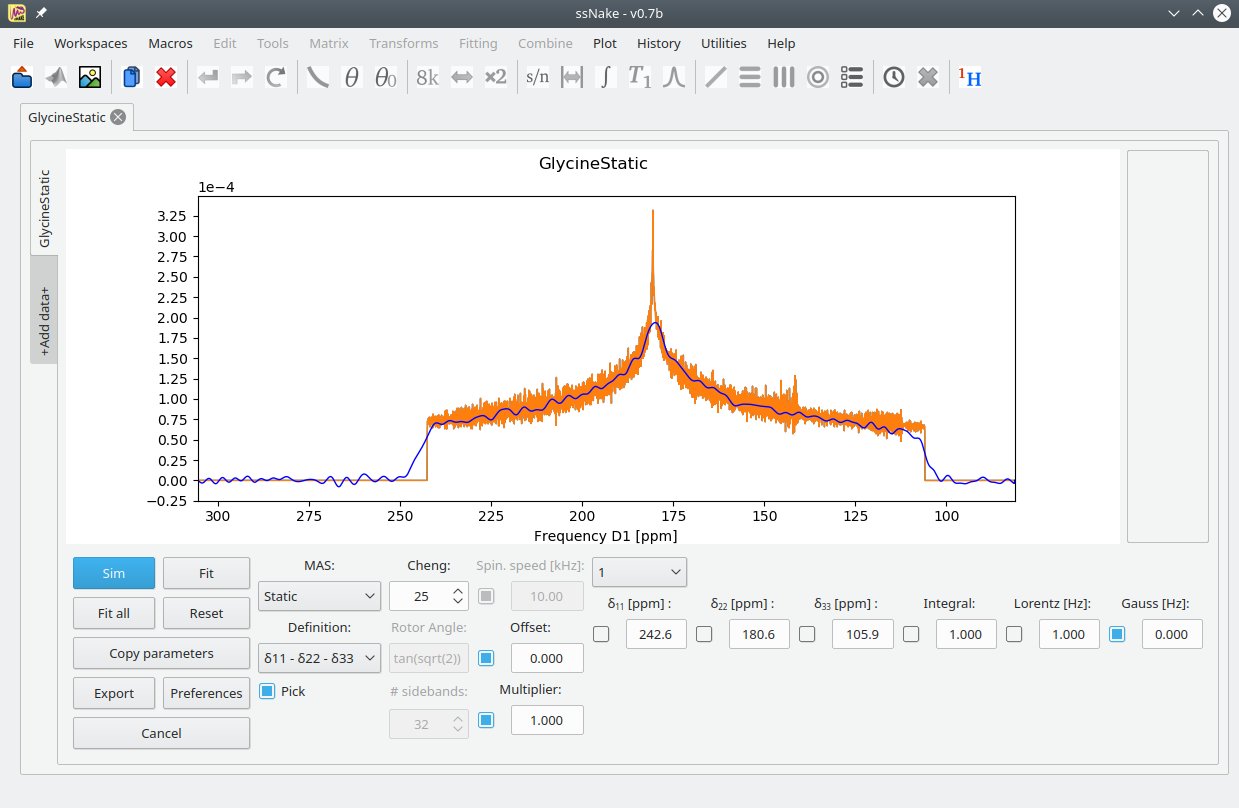
\includegraphics[width=0.8\linewidth]{Figs/Fig4.png}
\end{center}
which looks a lot more like a powder pattern. However, with Cheng at 25, the simulation starts to
become slower due to the high amount of orientations. In this case we actually do not need so many
orientations: our actual spectrum is not so precisely defined as there is significant
line broadening present (you can see this at the rounded edges of the pattern). Adding line
broadening to the simulations also means we need less powder orientations:
\begin{itemize}
  \item Set Cheng back to 15
  \item Set Lorentz at 500 Hz
\end{itemize}
Pushing `Sim' gives:
\begin{center}
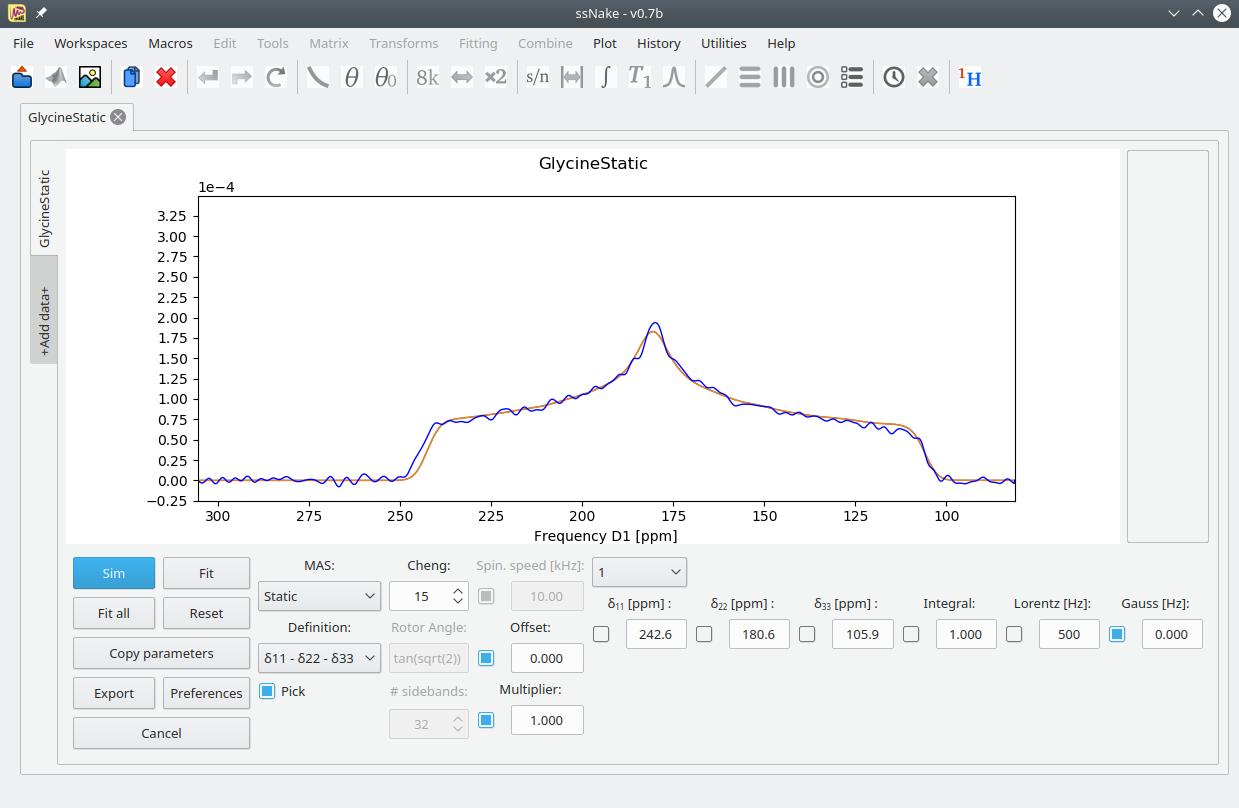
\includegraphics[width=0.8\linewidth]{Figs/Fig5.png}
\end{center}
which is quite close to the experimental spectrum.

We are now ready to let ssNake do some iterative fitting, to achieve the best description of our
spectrum. Push `Fit' to let it work its magic. This leads to the final fit:
\begin{center}
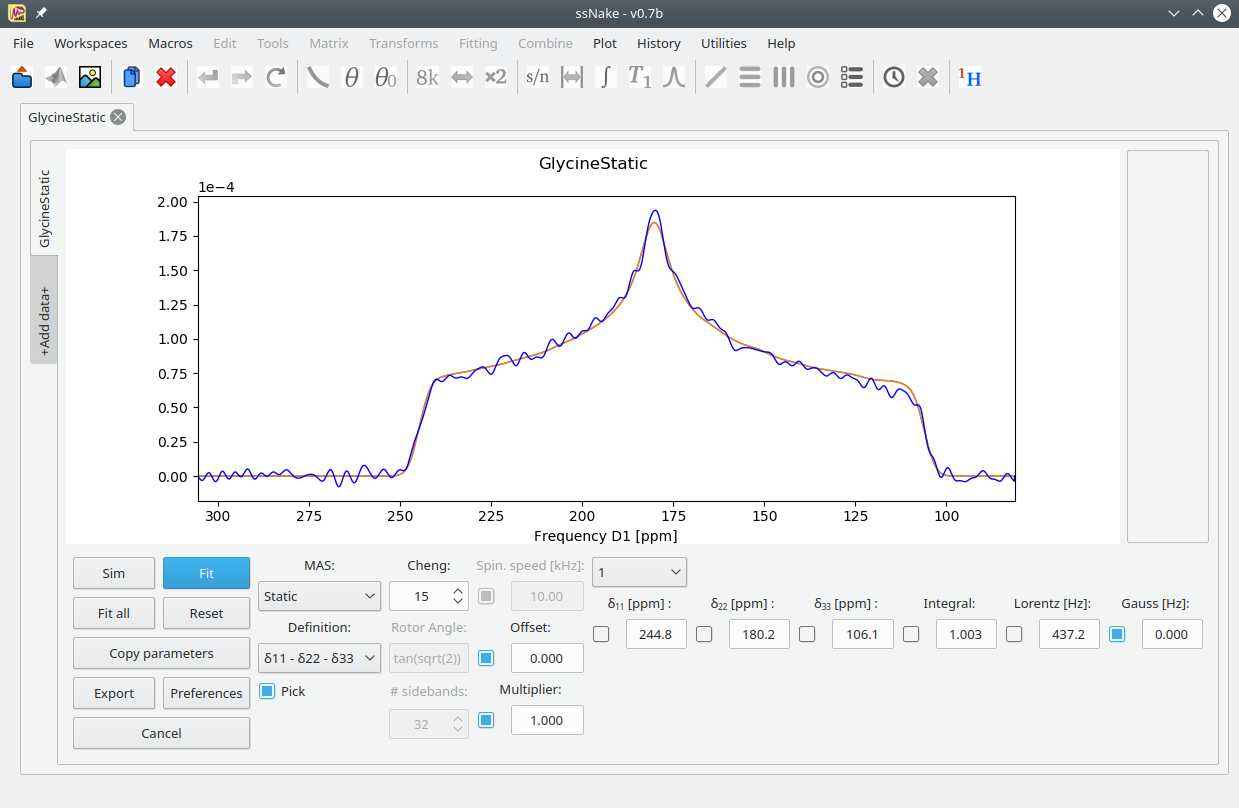
\includegraphics[width=0.8\linewidth]{Figs/Fig6.png}
\end{center}
with tensor values 244.8, 180.2, and 106.1 ppm. Often, the CSA tensor values are expressed in
another definitions. Common is the iso-aniso-eta definition. We can tell ssNake we need these values
by switching the definition from $\delta_{11}$--$\delta_{22}$--$\delta_{33}$ to
$\delta_\text{iso}$--$\delta_\text{aniso}$--$\eta$. ssNake automatically converts the tensor values on
the right. This gives 177.0, $-70.93$, and 0.9107. Using these other definitions can also be
convenient during fitting, for example in cases were you known $\delta_\text{iso}$ or $\eta$, and you
want to fix these values during the fit. Do note that in some definitions the mouse cannot be used
to sets values by clicking in the spectrum.

\end{document}
